\chapter{Non conforming and mixed Finite Element methods}

\section{Variational crimes}

We introduce here a framework that can be used when the hypothesis of the conforming finite element methods breakdown, either because the discretisation space $V_h$ is not included in the space  $V$where the variational formulation to be approximated is defined, or when the discrete bilinear form and the discrete linear form are not exactly the same the continuous ones.


We  consider the variational formulation: \emph{Find $u\in V$ such that}
\begin{equation}\label{eq:cont_non_conf}
 a(u,v) = l(v)\quad\forall v\in V.
 \end{equation}

In some cases it can be convenient to relax the constraints of the approximation space being a subspace of $V$ or to slightly modify the bilinear and linear form, using for example quadrature rules to compute the integrals or adding penalty terms. Let us then consider a mesh dependent family of Hilbert spaces $H_h$ equipped with a mesh dependent norm $\|\cdot\|_h$ such that $V \subset H_h$ and also $V_h\subset H_h$ for all $h$. One could choose $H_h=V+V_h$, but often some additional regularity of the exact solution is needed. Then one can choose $H_h=V\cap H^m(\Omega)+V_h$, where $H^m$ is a Sobolev space of the needed regularity.
  We then define the bilinear form $a_h$ on $H_h$ as an approximation of the bilinear form $a$ on $V$, and 
$l_h$ a linear form on $H_h$ approximating $l$ the linear form on $V$. We assume that $a_h$ and $l_h$ are continuous and that $a_h$ is uniformly coercive on $H_h$, meaning that the coercivity constant does not depend on $h$, even though the norm itself can depend on $h$.

As a typical example, given a subdivision of the domain $\Omega$ into elements
$\Omega = \cup K_e$ we can define 
$$H_h=\{ v \in L^2(\Omega) \;|\; v_{|K_e}\in H^1(K_e)\}, ~~~~~\mbox{ with } \|v\|_h^2 = \sum_{e}  \int_{K_e} |\nabla v(x)|^2 \dd x.$$
This is a broken $H^1$ space. Its elements are locally $H^1$ but not globally. Obviously $ V=H^1(\Omega)\subset H_h$. For $a(u,v)= \int_\Omega \nabla u(x) \cdot \nabla v(x) \dd x$ and  for a given $f\in L^2(\Omega)$,
$l(v) = \int_\Omega f(x)v(x) \dd x$, we define the approximations on $H_h$ by
$$a_h(u,v) = \sum_{e}  \int_{K_e} \nabla u(x)\cdot \nabla v(x) \dd x.$$
On the other hand $l$ is well defined on $H_h$ so that we can take $l_h=l$.
Obviously for $u,v\in V$, we have $a_h(u,v)=a(u,v)$ and $l_h(v)=l(v)$.

In this setting, we consider a discrete variational formulation of the following form:\\
\emph{  Find $u_h\in V_h$ such that}
\begin{equation}\label{eq:disc_non_conf}
 a_h(u_h,v_h) = l_h(v_h) \quad\forall v_h\in V_h.
\end{equation}

The error estimation of such an approximate variational formulation depends on the following lemma, known as Strang's second lemma \cite{strang-fix}, which replaces C\'ea's lemma:
\begin{lemma}[Strang]\label{lemma:strang2}
Assume $u\in V$ is the solution of \eqref{eq:cont_non_conf} and $u_h\in V_h$ its  approximation, solution of \eqref{eq:disc_non_conf}, then
\begin{equation}\label{eq:err_non_conf}
\|u-u_h\|_h \leq C \left(\inf_{v_h\in V_h} \|u-v_h\|_h + \sup_{v_h\in V_h} \frac{|a_h(u,v_h)-l_h(v_h)|}{\|v_h\|_h} \right).
\end{equation}
\end{lemma}
Note that as $u_h$ verifies $a_h(u_h,v_h) = l_h(v_h)$, we also could write 
$a_h(u,v_h)-l_h(v_h)=a_h(u-u_h,v_h)$.
\begin{remark}
The difference between C\'ea's Lemma that is used for the conforming approximation and the above Strang Lemma used for non conforming approximation is the presence of the second term on the right-hand-side, which is a consistency term, measuring how accurately the continuous solution verifies the discrete equation. This term vanishes when  $V_h\subset V$ and $a_h=a$ because of the Galerkin orthogonality.
\end{remark}
\begin{proof}
By bilinearity of $a_h$, we have
$$a_h(v_h-u_h,v_h-u_h)=a_h(v_h-u+u-u_h,v_h-u_h)=a_h(v_h-u,v_h-u_h) + a_h(u-u_h,v_h-u_h)$$
and also
\begin{align*}
a_h(u-u_h,v_h-u_h) &=  a_h(u,v_h-u_h)- a_h(u_h,v_h-u_h), \\
&=   a_h(u,v_h-u_h)  - l_h(v_h-u_h),
\end{align*}
as $u_h$ verifies \eqref{eq:disc_non_conf}.

Using the uniform coercivity and continuity of $a_h$ in $H_h$,
there exists  $\alpha>0$ and $\beta$ such that for any $v_h\in V_h$
\begin{align*}
  \alpha \|v_h-u_h\|_h^2 &\leq a_h(v_h-u_h,v_h-u_h) 
 \leq  a_h(v_h-u,v_h-u_h) + a_h(u-u_h,v_h-u_h)
  \\
  &\leq a_h(v_h-u,v_h-u_h) +  a_h(u,v_h-u_h) -  l_h(v_h-u_h),\\
  &\leq \beta\|v_h-u\|_h\|v_h-u_h\|_h +  \frac{|a_h(u,v_h-u_h)-l_h(v_h-u_h)|}{\|v_h-u_h\|_h}
  \|v_h-u_h\|_h
\end{align*}
as $a_h$ is continuous.
Whence 
$$\|v_h-u_h\|_h\leq \frac \beta\alpha \|u-v_h\|_h
+\frac{1}{\alpha}\sup_{v_h\in V_h}  \frac{|a_h(u,v_h)-l_h(v_h)|}{\|v_h\|_h}
$$ for all
$v_h\in V_h$. This combined with  the triangle inequality yields
$$\|u-u_h\|_h\leq \|u-v_h\|_h + \|v_h-u_h\|_h \leq
\left(1+\frac{\beta}{\alpha} \right)\|u-v_h\|_h
+\frac{1}{\alpha}\sup_{v_h\in V_h}  \frac{|a_h(u,v_h)-l_h(v_h)|}{\|v_h\|_h}.
$$
We then get the desired results taking the infimum in $V_h$.
\end{proof}

\section{Non conforming $ \mathbb{P}_k$ finite elements on triangles}

Let us consider the Poisson equation with Dirichlet boundary conditions given $f\in L^2(\Omega)$, for which the variational formulation reads: \emph{ Find $u\in H^1_0(\Omega)$ such that}
\begin{equation}\label{eq:poisson_nonconf}
\int_\Omega \nabla u\cdot \nabla v \dd \mathbf{x} = \int_\Omega f v \dd \mathbf{x}\quad\forall v\in H^1_0(\Omega).
\end{equation}

Standard conforming $\mathbb{P}_k$ finite elements on triangles have $k+1$ points on each
edge, which are shared between elements to enforce continuity. 
Let us now consider the case, when only $k$ points are put on each side. 
The corresponding non conforming $ \mathbb{P}_1$ and $ \mathbb{P}_3$ elements are displayed on figure \ref{fig:non_conf}. They are also known as Crouzeix-Raviart Finite Elements.
\begin{figure}[htbp]
\centerline{
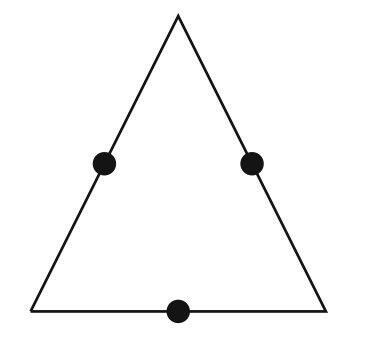
\includegraphics[width=.3\textwidth]{figures/part_4/P1_non_conf} ~~~~~~~
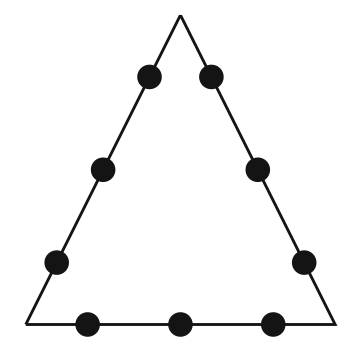
\includegraphics[width=.3\textwidth]{figures/part_4/P3_non_conf} 
}
\caption{\label{fig:non_conf} Non conforming $ \mathbb{P}_1$ (left) and $ \mathbb{P}_3$ (right) Finite Elements. }
\end{figure}
This is not enough to get continuity across the element and thus conformity, but is it still possible to define an optimal approximation? This is the case if the error coming from the second term in the second Strang Lemma is of the same order as the polynomial approximation error with $ \mathbb{P}_k$ elements, \textit{i.e.} \mbox{$\|u-u_h\|_h\leq C h^{k}$}. This can be obtained by putting the degrees of freedom on each edge at the Gauss points. Note however that this works only for $k$ odd, as for $k$ even the degrees of freedom obtained in this way are not linearly independent.

Consider the Lagrange Finite Element $(K_e,P_e,\Sigma_e)$, and $(a_i)_{i=1,N}$ the set of all degrees of freedom on all elements. As usual these degrees of freedom are shared by elements having an edge in common, but in the non-conforming case we are considering this is not enough to ensure continuity. The approximation space is then naturally defined as follows:
\begin{multline*}
V_h=\{ v_h\in L^2(\Omega) \;|\; v_{h|K_e}\in \mathbb{P}_k, v_{h|K_{e_1}}(a_i) =   v_{h|K_{e_2}}(a_i) \mbox{ if }a_i\in K_{e_1}\cap K_{e_2}, \\
v_h(a_i)=0  \mbox{ if } a_i \mbox{ on }\partial\Omega\}.
\end{multline*}

As  $V_h \not\subset H^1_0(\Omega)$, we cannot directly use the variational formulation\eqref{eq:poisson_nonconf}. Instead we use its "broken" version:
\emph{Find $u_h \in V_h $ such that}
\begin{equation}\label{eq:poisson_nonconf}
\sum_e \int_{K_e} \nabla u_h\cdot \nabla v_h \dd \mathbf{x} = \int_\Omega f v_h \dd \mathbf{x}\quad\forall v_h\in V_h.
\end{equation}
We then are in the abstract framework defined above with
$$a_h(u_h,v_h)=\sum_e \int_{K_e} \nabla u_h\cdot \nabla v_h \dd \mathbf{x} , ~~~~
l_h(v_h)=l(v_h) = \int_\Omega f v_h \dd \mathbf{x}.$$
Let us now express the consistency error in this non-conforming approximation. Let $u\in H^1_0(\Omega)\cap H^2(\Omega)$ be the exact solution of \eqref{eq:poisson_nonconf} and $v_h\in V_h$, then
\begin{align}
a_h(u,v_h)-l_h(v_h)&= 
\sum_e \int_{K_e} \nabla u \cdot \nabla v_h \dd \mathbf{x} - \int_\Omega f v_h \dd \mathbf{x} \\
&= -\sum_e \left[\int_{K_e} (\Delta u +f) \cdot  v_h \dd \mathbf{x} - \int_{\partial{K_e}} \fracp{u}{n} v_h \dd \sigma \right] \\
&= \sum_e \int_{\partial{K_e}} \fracp{u}{n} v_h \dd \sigma
\end{align}
as $u$ verifies $-\Delta u =f$. 

For two adjacent elements  $K_{e_1}$ and $K_{e_2}$ let us denote by $\Gamma_s=  K_{e_1}\cap K_{e_2}$ their shared edge.
Let  $v_s$ be the interpolation of polynomial of degree $k-1$ of $v_{h|K_{e_1}}$ and $v_{h|K_{e_2}}$ at the degrees of freedom on the edges of the two elements. As the degrees of freedom are shared by elements sharing the same edge, $v_s$ is the same on the two elements $K_{e_1}$ and
$K_{e_2}$. Then as the unit outward normal for these two elements has opposite signs on $\Gamma_s$, it follows that
$$ \int_{\Gamma_s} \fracp{u}{n_{e_1}} v_s \dd \sigma + \int_{\Gamma_s} \fracp{u}{n_{e_2}} v_s \dd \sigma=0.$$
On the other hand if $\Gamma_s$ corresponds to a boundary of $\Omega$ the degrees of freedom there are set to zero, so that $v_s=0$ on such a boundary.
Hence adding the contributions over the whole mesh
$$a_h(u,v_h)-l_h(v_h) =  \sum_e \int_{\partial{K_e}} \fracp{u}{n} (v_h-v_s) \dd \sigma. $$
Let us now introduce $\pi_h u$, the Finite Element interpolant of $u$, which is by definition a polynomial of degree $k$ on each element. Then $ \fracp{\pi_h u}{n} $ is a polynomial of degree $k-1$ on the edges of the mesh. So if, the degrees of freedom are chosen to be Gauss points on the edges,
$v_h-v_s$ on each edge is a polynomial of degree $k$ having its zeros at the Gauss points. Hence it is, up to a multiplicative constant, the Legendre polynomial of degree $k$, which is orthogonal to all polynomials of degree $k-1$. Thus for all edges
$$ \int_{\Gamma_s} \fracp{\pi_h u}{n} (v_h-v_s) \dd \sigma = 0.$$
Adding the contributions over the whole mesh it follows that
\begin{align*}
a_h(u,v_h)-l_h(v_h) &=  \sum_e \int_{\partial{K_e}} \left(\fracp{u}{n}-\fracp{\pi_h u}{n}\right)  (v_h-v_s) \dd \sigma \\
&\leq C \sum_e \|\nabla (u-\pi_h u)\cdot \mathbf{n}\|_{L^2(\partial{K_e})} \| v_h-v_s \|_{\partial{K_e})},
\end{align*}
using a Cauchy-Schwartz inequality. Then we can use the polynomial approximation properties on mesh faces as proved in \cite{dipietro2012} (Lemma 1.59, p. 32), assuming $u\in H^{k+1}(\Omega)$ with $k\geq 1$
\begin{equation}\label{eq:pol_approx_edge}
 \|\nabla (u-\pi_h u)\cdot \mathbf{n}\|_{L^2(\partial{K_e})}  \leq C h^{k-1/2} |u|_{k+1,K_e}, ~~~~
  \| v_h-v_s \|_{\partial{K_e})} \leq C h^{k-1/2} |v_h|_{k+1,K_e}, 
\end{equation}
$\pi_h u$ being a polynomial of degree $k$ approximating $u$ and $v_s$ a polynomial of degree $k-1$ approximating $v_h$.
Then it follows 
$$\frac{|a_h(u,v_h)-l_h(v_h) |}{\|v_h\|_h} \leq C  \sum_e h^{k-\frac 12} |u|_{k+1,K_e} h^{k-\frac 12} \leq C h^k |u|_{k+1,\Omega},$$
as $k\geq 1$.


\section{Weak enforcement of Dirichlet boundary conditions}

Another useful application of non conforming finite element is the weak enforcement of Dirichlet conditions following an idea of Nitsche \cite{nitsche1971}. We consider here a standard Finite Element conforming in $H^1$ (for the Poisson problem) but not in $H^1_0$. 

Let us explain the method for the Poisson problem with Dirichlet boundary conditions. Here because the vector space where the solution lives is $H^1(\Omega)$ anyway, as for natural boundary conditions, non homogeneous boundary conditions are as easy to enforce as homogeneous boundary conditions. Our problem then reads
$$-\Delta u= f ~~~ \mbox{ in } \Omega, ~~~~ u=g ~~~~\mbox{ on } \partial \Omega.$$
In order to get a consistent variational formulation,
as usual in the derivation of the Finite Element method we multiply the first equation by a test function $v$ and integrate on the whole domain
\begin{align*}
-\int_\Omega \Delta u v \dd \mathbf{x} &= \int_\Omega f v  \dd \mathbf{x} \\
& = \int_\Omega \nabla u \cdot \nabla v \dd \mathbf{x} - \int_{\partial \Omega} \fracp{u}{n} v \dd \sigma
\end{align*}
In the standard conforming Finite Element method the boundary integral vanishes by taking test functions vanishing on the boundary.  Instead here we keep it, moreover so that the problem remains symmetric, we add $\int_{\partial \Omega} u \fracp{v}{n} \dd \sigma$, which is known as $u$ the exact solution is equal to a known function $g$  on the boundary. 
Then the exact solution of our problem satisfies the following relation
\begin{equation}\label{eq:nitsche_sym}
\int_\Omega \nabla u \cdot \nabla v \dd \mathbf{x} 
- \int_{\partial \Omega} \fracp{u}{n} v \dd \sigma -\int_{\partial \Omega} u \fracp{v}{n} \dd \sigma =
 \int_\Omega f v  \dd \mathbf{x}  -\int_{\partial \Omega} g \fracp{v}{n}\dd\sigma \quad\forall v\in H^1 (\Omega).
 \end{equation}
 The left-hand-side defines a symmetric bilinear form, but it is not coercive and thus does not lead to a well posed variational problem. 
 
However, we can use this relation to define a consistent discrete variational problem. In order to make it coercive, we need to add an additional term $\mu_h \int_{\partial \Omega} u_h v_h \dd \sigma$, called penalty term which will be grid dependent, that vanishes for the exact solution and $\mu_h$ will be chosen such that the resulting bilinear form is coercive in some norm. 
For this we define the standard Lagrange approximation space for $H^1(\Omega)$
$$V_h=\{ v_h\in C^0(\Omega) \;|\; v_{h|K_e}\in \mathbb{P}_k(K_e)\},$$
and then the discrete variational problem reads: \emph{Find $u_h\in V_h$ such that}
\begin{multline*}
\int_\Omega \nabla u_h \cdot \nabla v_h \dd \mathbf{x} +\mu_h\int_{\partial \Omega} u_h v_h \dd \sigma
- \int_{\partial \Omega} \fracp{u_h}{n} v_h \dd \sigma -\int_{\partial \Omega} u_h \fracp{v_h}{n} \dd \sigma \\ =
 \int_\Omega f v_h  \dd \mathbf{x} -\int_{\partial \Omega} g \fracp{v_h}{n}\dd\sigma +\mu_h \int_{\partial \Omega} g v_h\dd\sigma \quad\forall v_h\in V_h.
\end{multline*}
This corresponds to an abstract mesh depend variational problem of the form:\\
 \emph{Find $u_h\in V_h$ such that}
$a_h(u_h,v_h)=l_h(v_h), ~~\forall v_h\in V_h$, with
\begin{align*}
a_h(u_h,v_h) &= \int_\Omega \nabla u_h \cdot \nabla v_h \dd \mathbf{x} +\mu_h\int_{\partial \Omega} u_h v_h \dd \sigma
- \int_{\partial \Omega} \fracp{u_h}{n} v_h \dd \sigma -\int_{\partial \Omega} u_h \fracp{v_h}{n} \dd \sigma \\
l_h(v_h) &=  \int_\Omega f v_h  \dd \mathbf{x} -\int_{\partial \Omega} g \fracp{v_h}{n}\dd\sigma
+\mu_h \int_{\partial \Omega} g v_h\dd\sigma.
\end{align*}

Because $V_h\subset H^1(\Omega)$, we can take in equation \eqref{eq:nitsche_sym} $u$ to be the exact solution and $v=v_h\in V_h$. Then as in addition the exact solution $u$ is equal to $g$ on the boundary, the consistency error appearing in the second Strang Lemma (Lemma \ref{lemma:strang2}) vanishes completely:
$$a_h(u,v_h) - l_h(v_h) = 0 \quad\forall v_h\in V_h.$$

We can now prove a lemma giving a condition on the penalisation parameter $\mu_h$ such that the bilinear form $a_h$ is coercive in the mesh depend norm 
$$\|v \|_h^2 =  \|\nabla v \|_{0,\Omega}^2 + \frac{1}{h} \| v \|_{0,\partial\Omega}^2\quad\forall v\in H^1(\Omega).$$ 
\begin{lemma}
Assume that there exists $C>0$ such that $\|\nabla v\|_{0,\partial\Omega} \leq C h^{-1/2} \|\nabla v\|_{0,\Omega}$ then the bilinear form $a_h$ is uniformly coercive in  the mesh dependent norm $\|\cdot\|_h$ if $\mu_h =\alpha/h$ with  $\alpha > 2C^2 $.
\end{lemma}
\begin{proof}
Let us first observe that for any $v\in H^1(\Omega)$
$$a_h(v,v)= \|\nabla v\|_{0,\Omega}^2 + \mu_h\| v\|_{0,\partial\Omega}^2
- 2 \int_{\partial \Omega} \fracp{v}{n} v \dd \sigma=
 \|\nabla v\|_{0,\Omega}^2 + \frac{\alpha}{h}\| v\|_{0,\partial\Omega}^2
- 2 \int_{\partial \Omega} \fracp{v}{n} v \dd \sigma.$$
Then, using the Cauchy-Schwarz inequality, the fact that the components of the normal vector are less than one, and the assumption of the Lemma
$$ 2\int_{\partial \Omega} \fracp{v}{n} v \dd \sigma \leq  2\|\nabla v\|_{0,\partial \Omega}
\|v\|_{0,\partial\Omega} 
\leq   2C h^{-1/2} \|\nabla v\|_{0,\Omega} \|v\|_{0,\partial\Omega} 
\leq \frac 12 \|\nabla v\|_{0,\Omega}^2 +  \frac{2C^2}{h} \|v\|_{0,\partial\Omega}^2
$$
using also for the last inequality the property $ab \leq a^2/2 + b^2/2$ for any real numbers $a,b$.
Plugging the opposite inequality into the expression of $a_h(v,v)$ we get
$$a_h(v,v) \geq \frac 12 \|\nabla v\|_{0,\Omega}^2  +  \frac{\alpha -  2C^2}{h} \|v\|_{0,\partial\Omega}^2
\geq \min ( \frac 12, \alpha -  2C^2 ) (   \|\nabla v\|_{0,\Omega}^2  + \frac 1h\|v\|_{0,\partial\Omega}^2) .$$
This yields the uniform coercivity of $a_h$ in the mesh dependent norm provided $\alpha> 2C^2 $.
\end{proof}

\begin{remark}
In practical applications, it is best to choose $\mu_h$ not too much larger than the minimal value needed for coercivity. This can be achieved for a given mesh, by solving the generalized eigenvalue problem 
$$ \int_\Omega \nabla u_h \cdot \nabla v_h \dd \mathbf{x} 
- \int_{\partial \Omega} \fracp{u_h}{n} v_h \dd \sigma -\int_{\partial \Omega} u_h \fracp{v_h}{n} \dd \sigma = \lambda_h\int_{\partial \Omega} u_h v_h \dd \sigma \quad\forall v_h \in V_h
$$
which can be written in matrix form, once the Finite Element matrices are assembled
$A U = \lambda_h BU$. The matrices being symmetric, all eigenvalues are real, and the smallest one denoted by $\lambda_{h,0}$ should be negative because of the lack of coercivity.
In order to get coercivity then one needs to choose $\mu_h > |\lambda_{h,0}|$. 
If one chooses $\mu_h = \alpha  |\lambda_{h,0}|$ with $\alpha$ a coefficient independent of $h$ typically between 1 and 2, one gets the optimal order of convergence.
\end{remark}



\section{Discontinuous Galerkin methods}

The Nitsche method to weakly enforce Dirichlet boundary conditions also inspired researchers for getting rid of the conformity at element interfaces using the idea of writing a consistent approximation involving the interface terms, then symmetrizing and penalizing to get a symmetric and coercive mesh dependent form. This leads to the so-called SIP (symmetric interior penalty) Discontinuous Galerkin (DG) method that was introduced, adapting previous works, and analyzed by Arnold \cite{arnold1982}. See also \cite{arnold2002} for a historical and more general discussion on Discontinuous Galerkin methods. A mathematical textbook presentation of the discontinuous Galerkin method can be found for example in \cite{dipietro2012}.

Let us explain the method on the Poisson equation with homogeneous Dirichlet boundary conditions.
$$-\Delta u= f ~~~ \mbox{ in } \Omega, ~~~~ u=0 ~~~~\mbox{ on } \partial \Omega.$$



Instead of multiplying by a smooth function over the whole domain as in the classical finite element method, we here introduce the mesh first $\mathcal{T}_h= \cup_e K_e$. Let $v_h\in L^2(\Omega)$ such that $v_h\in H^1(K_e)$. In practice $v_h$  will be polynomial or in a local Finite Element space. Let us denote by $n_e$ the outward unit normal for element $K_e$ and denoting by
$(\Gamma_s)_s$ the edges of the grid, $\Gamma_s=K_{e_1}\cap K_{e_2}$, by $n_s$ a unit normal to the edge $\Gamma_s$ (the sign being arbitrarily chosen so that $n_s=n_{e_1}$). As usual in Discontinuous Galerkin formulations we denote by
$\lav v \rav= (v_{|K_{e_1}} + v_{|K_{e_2}})/2$ the average of $v$ on the edge $\Gamma_s$ and
$\ljump v \rjump= v_{|K_{e_1}} - v_{|K_{e_2}}$ the jump of $v$ on the edge $\Gamma_s$. For edges on the boundary of the domain, we assume that the outside value is zero so that $\lav v \rav = \ljump v \rjump= v$. Then, we multiply by a smooth function $v_{h|K_e}$ on one element, integrate over this element and sum over all the elements
\begin{align}
\sum_e \int_{K_e} (-\Delta u) v_h \dd \mathbf{x} &=  
\sum_e  \left[ \int_{K_e}\nabla u \cdot \nabla v_h \dd \mathbf{x} 
-  \int_{\partial{K_e}} \fracp{u}{n_e}  v_h \dd \sigma  \right] \nonumber\\
&=  
\sum_e  \int_{K_e}\nabla u \cdot \nabla v_h \dd \mathbf{x} 
- \sum_s  \int_{\Gamma_s}\fracp{u}{n_s}\ljump v_h \rjump \dd \sigma  \nonumber\\
&= \sum_e  \int_{K_e}\nabla u \cdot \nabla v_h \dd \mathbf{x} 
- \sum_s  \int_{\Gamma_s}\lbav \fracp{u}{n_s}\rbav\ljump v_h \rjump \dd \sigma 
\label{eq:sip_consist}
\end{align}
as the exact solution, which is in $H^2$, has a continuous normal derivative across the edges, this is equal to its average.

This formula can be used to get a consistent approximation. As for the Nitsche method we now symmetrize and penalize the interface jumps. We then get the mesh dependent bilinear form
\begin{multline}\label{eq:sip_ah}
a_h(u_h,v_h) =  \sum_e  \int_{K_e}(\nabla u \cdot \nabla v_h) \dd \mathbf{x} 
- \sum_s  \int_{\Gamma_s}\lbav \fracp{u_h}{n_s}\rbav\ljump v_h \rjump \dd \sigma 
-\sum_s   \int_{\Gamma_s}\ljump u_h \rjump\lbav \fracp{v_h}{n_s}\rbav \dd \sigma \\
+\mu_h  \int_{\Gamma_s}\ljump u_h \rjump\ljump v_h\rjump \dd \sigma. 
\end{multline}
Then, defining the linear form
$$l_h(v_h) = \int_\Omega f v_h \dd \mathbf{x} =   \sum_e  \int_{K_e}f v_h \dd \mathbf{x}  $$
 and the discontinuous polynomial space
$$V_h=\{ v_h\in L^2(\Omega) \;|\; v_{h|K_e}\in \mathbb{P}_k(K_e) \},$$
 the discrete variational formulation for our problem reads: \emph{Find $u_h\in V_h$ such that }
\begin{equation}\label{eq:dg_sip}
a_h(u_h,v_h) = l_h(v_h) \quad\forall v_h\in V_h.
\end{equation} 
As the exact solution $u$ is continuous, the jump of $u$ at the element interfaces vanishes, \textit{i.e.}
$\ljump u \rjump=0$, hence the two last terms in \eqref{eq:sip_ah}, which are respectively the symmetry term and the penalty term vanish for $u_h=u$. Hence using the calculation \eqref{eq:sip_consist} we can verify that the consistency error in the DG-SIP method \eqref{eq:dg_sip} is exactly vanishing:
$$a_h(u,v_h) - l_h(v_h) = \sum_e \int_{K_e} (-\Delta u) v_h \dd \mathbf{x} - \int_\Omega f v_h \dd \mathbf{x} = -\int_\Omega (\Delta u+f) v_h \dd \mathbf{x} = 0$$
as $-\Delta u=f$.

Even though they are not conforming as $V_h\not\subset V$, DG methods are build to be exactly consistent, so that the consistency error in the second Strang lemma \ref{lemma:strang2} exactly vanishes. The error analysis described in the book by Di Pietro and Ern \cite{dipietro2012} relies on this property. See in particular Section 4.2, which provides a convergence analysis of the SIP-DG method in an \textit{ad hoc} mesh dependent norm, following the same pattern as for the Nitsche method. 

\section{Saddle-point problems}

\subsection{The theoretical framework} 

The variational problems we consider here fit into the following framework. 
Consider two Hilbert spaces $V$ and $W$, two continuous bilinear forms
$a\in \mathcal{L}(V\times V, \mathbb{R})$ and $b\in \mathcal{L}(V\times W, \mathbb{R})$
and two continuous linear forms $l_V\in \mathcal{L}(V, \mathbb{R})$ and
$l_W\in \mathcal{L}(W, \mathbb{R})$.
Then we defined the abstract mixed variational problem as {\em Find $(u,p)\in V\times W$ such that}
\begin{align}
a(u,v) + b(v,p) &= l_V(v) \quad \forall v\in V, \label{eq:abs_var_mixed1}\\
b(u,q) &= l_W(q) \quad \forall q\in W.  \label{eq:abs_var_mixed2}
\end{align}

For saddle point problems the Lax-Milgram framework cannot be applied. In this case the appropriate theoretical tool, called Banach-Ne\v{c}as-Babu\v{s}ka (BNB) theorem in Ern and Guermond, which is more general than Lax-Milgram. We will specialise it to our type of mixed problems assuming that the bilinear form $a$ is symmetric and coercive on $K=\{v\in V\; | \; b(q,v)=0,~\forall q\in W\}$. This corresponds to Theorem 2.34 p.~100 of \cite{ern2004}, modified according to Remark 2.35.


\begin{theorem} Let $V$ and $W$ be Hilbert space. Assume $a$ is a continuous bilinear form on
$V\times V$ and that b is a continuous linear form on $V\times W$, that  $l_V$ and $L_W$ are continuous linear forms on $V$  and $W$ respectively and that the following two hypotheses are verified
\begin{itemize}
\item[1)]  $a$ is coercive on $K=\{v\in V\; |\; b(q,v)=0,~\forall q\in W\}$, \textit{i.e.} there exists $\alpha>0$ such that
$$a(v,v) \geq \alpha \|v\|^2_V \quad\forall v\in K.$$
\item[2)] The Babuska-Brezzi, or inf-sup condition, is verified:  there exists $\beta>0$ such that
$$ \inf_{q\in W} \sup_{v\in V} \frac{b(v,q)}{\|q\|_W\|v\|_V} \geq \beta.$$
\end{itemize}
Then the variational problem admits a unique solution and the solution satisfies the a priori estimate
$$\|u\|_V \leq \frac{1}{\alpha} \|f\|_{V'} + \frac{1}{\beta}(1+ \frac{C}{\alpha})  \|g\|_{W'}, ~~~~
\|p\|_W \leq \frac{1}{\beta}(1+ \frac{C}{\alpha})  \|f\|_{V'} + \frac{C}{\beta^2}(1+ \frac{C}{\alpha})  \|g\|_{W'},$$
where $C$ is the continuity constant of $a$.
\end{theorem}

The inf-sup conditions  plays an essential role, as it is only satisfied if the spaces $V$ and $W$ are compatible in some sense. This condition being satisfied at the discrete level  with a constant $\beta$ that does not depend on the mesh size being essential for a well behaved Finite Element method.  It can be written equivalently
\begin{equation}\label{inf-sup}
\beta \|q\|_W \leq \sup_{v\in V} \frac{b(v,q)}{\|v\|_V} \quad \forall q\in W.
\end{equation}
And often, a simple way to verify it is, given any  $q\in W$, to find a specific $v=v(q)$ depending on $q$ such that
$$\beta \|q\|_W \leq \frac{b(v(q),q)}{\|v(q)\|_V} \leq \sup_{v\in V} \frac{b(v,q)}{\|v\|_V}$$ with a constant $\beta$ independent of $w$.


Let us now come to the Galerkin discretisation. The principle is simply to construct finite dimensional subspaces $W_h \subset W$ and $V_h\subset V$ and to write the variational formulation \eqref{eq:abs_var_mixed1}-\eqref{eq:abs_var_mixed2} replacing $W$ by $W_h$ and $V$ by $V_h$. 
The variational formulations are the same as in the continuous case, like for conforming finite elements. This automatically yields the consistency of the discrete formulation.
In order to get the stability property needed for convergence, we need that the coercivity constant $\alpha$ and the inf-sup constant $\beta$ are independent of $h$.

Because $V_h\subset V$ the coercivity property is automatically verified in the discrete case, with a coercivity constant that is the same as in the continuous case and hence does not depend on the discretisation parameter $h$.

Here, however, there is an additional difficulty, linked to the inf-sup conditions, which is completely dependent on the two spaces $V_h$ and $W_h$. By far not any conforming approximation of the two spaces will verify the discrete inf-sup condition with a constant $\beta$ that is independent on $h$. Finding compatible discrete spaces for a given mixed variational formulation, has been an active area of research. 

 
%A nice framework to have this compatibility condition verified is the exact sequence of discrete spaces, thanks to which it is always possible to find for any $q$ a $v$ in the previous space such that $Av=q$.





\subsection{Mixed formulation of the Poisson problem}

Consider the Poisson problem
\begin{align}
-\Delta p & =f  \label{eq:poisson_mixed}\\
p& =0
\end{align}
Using that $\Delta p = \nabla\cdot\nabla p$, we set $ \mathbf{u}=\nabla p$, then the Poisson equation \eqref{eq:poisson_mixed} can be written equivalently
$$ \mathbf{u}=-\nabla p, ~~~ \nabla\cdot \mathbf{u}= f.$$
Instead of having one unknown, we now have two, along with the above two equations.
In order to get a mixed variational formulation, we first take the dot product of the first one by $ \mathbf{v}$ and integrate by parts
$$\int \mathbf{u}\cdot \mathbf{v}\dd \mathbf{x} -\int p\,\nabla\cdot \mathbf{v}\dd \mathbf{x} +
\int_{\partial\Omega} p \,  \mathbf{v}\cdot \mathbf{n}\dd \sigma=
\int \mathbf{u}\cdot \mathbf{v}\dd \mathbf{x} -\int p\,\nabla\cdot \mathbf{v}\dd \mathbf{x}=0,$$
using $p=0$ as a natural boundary condition. Then multiplying the second equation by $q$ and integrating yields
$$\int \nabla\cdot\mathbf{u} \, q \dd \mathbf{x} = \int f q \dd \mathbf{x}.
$$
No integration by parts is necessary here. And we thus get the following mixed variational formulation:
{\em Find $(\mathbf{u},p) \in H(\operatorname{div},\Omega)\times L^2(\Omega)$ such that}
\begin{align}
\int \mathbf{u}\cdot \mathbf{v}\dd \mathbf{x} -\int p\,\nabla\cdot \mathbf{v}\dd \mathbf{x}&=0 \quad \forall \mathbf{v}\in H(\operatorname{div},\Omega) \\
\int \nabla\cdot\mathbf{u} \, q \dd \mathbf{x} & = \int f q \dd \mathbf{x}, \quad \forall q\in L^2(\Omega).
\end{align}

Here also, we get an alternative formulation by not integrating by parts, the mixed term in the first formulation but in the second. The first formulation simply becomes
$$\int \mathbf{u}\cdot \mathbf{v}\dd \mathbf{x} +\int \nabla p \cdot \mathbf{v}\dd \mathbf{x}=0,$$
and the second, removing immediately the boundary term due to the essential boundary condition $q=0$
$$\int\nabla \cdot\mathbf{u}  \, q \dd \mathbf{x} =
 -\int  \mathbf{u} \cdot \nabla q  \dd \mathbf{x} =
\int f q \dd \mathbf{x},$$
which leads to the variational formulation
{\em Find $(\mathbf{u},p) \in L^2(\Omega)^3 \times H^1_0(\Omega)$ such that}
\begin{align}
\int \mathbf{u}\cdot \mathbf{v}\dd \mathbf{x} +\int \nabla p \cdot \mathbf{v}\dd \mathbf{x}&=0 \quad \forall \mathbf{v}\in L^2(\Omega)^3 \\
\int  \mathbf{u} \cdot \nabla q  \dd \mathbf{x} & = -\int f q \dd \mathbf{x}, \quad \forall q\in H^1_0(\Omega).
\end{align}
Note that this formulation actually contains the classical variational formulation for the Poisson equation. Indeed for $q\in H^1_0(\Omega)$, $\nabla q \in L^2(\Omega)^3$ can be used as a test function in the first equation. And plugging this into the second we get
$$\int  \nabla p \cdot \nabla q  \dd \mathbf{x}  = \int f q \dd \mathbf{x}, \quad \forall q\in H^1_0(\Omega).$$



%coercivity of $a$ trivial
%Inf-sup: take $p\in H_0^1$, $v=\nabla p\in L^2$, inf sup condition follows from Poincar\'e inequality.


%\subsection{The Stokes problem}
%
%We consider now the Stokes problem for the steady-state modelling of an incompressible fluid
%\begin{equation}\label{eq:stokes}
%-\Delta \mathbf{u} + \nabla p = \mathbf{f}, ~~~~ \nabla\cdot \mathbf{u}=0 \mbox{ in }\Omega,~~~~  \mathbf{u}=0, ~~p=0 \mbox{ on }\partial\Omega
%\end{equation}
%For the variational formulation, we take the dot product of the first equation with $v$ and integrate over the whole domain
%$$\int (-\Delta \mathbf{u} + \nabla p)\cdot \mathbf{v} \dd \mathbf{x} 
%=\int\nabla \mathbf{u}:\nabla \mathbf{v} \dd \mathbf{x} + \int \nabla p \cdot \mathbf{v} \dd \mathbf{x}
%= \int \mathbf{f}\cdot \mathbf{v} \dd \mathbf{x} =0.$$
%The integration by parts is performed component by component. We impose the essential boundary condition $ \mathbf{v}=0$ on $\partial\Omega$, and we denote by
%$$\int\nabla \mathbf{u}:\nabla \mathbf{v} \dd \mathbf{x} =\sum_{i=1}^3 \int\nabla u_i\cdot\nabla v_i \dd \mathbf{x} =\sum_{i,j=1}^3 \int\partial_j u_i\partial_j v_i \dd \mathbf{x} .$$
%We now need to deal with the constraint $\nabla\cdot \mathbf{u}=0$. The theoretical framework for saddle point problems requires that the corresponding bilinear form is the same as the second one appearing in the first part of the variational formulation. To this aim we multiply  $\nabla\cdot \mathbf{u}=0$ by a scalar test function (which will be associated to $p$) and integrate on the full domain, with an integration by parts in order to get the same bilinear form as in the first equation
%$$\int \nabla\cdot \mathbf{u} \,q \dd \mathbf{x}= - \int \mathbf{u}\cdot \nabla q\dd \mathbf{x}=0,$$
%using that $q=0$ on the boundary as an essential boundary condition.
%We finally obtain the mixed variational formulation: {\em Find $( \mathbf{u},p)\in H^1_0(\Omega)^3\times H^1_0(\Omega)$ such that }
% $$\int\nabla \mathbf{u}:\nabla \mathbf{v} \dd \mathbf{x} + \int \nabla p \cdot \mathbf{v} \dd \mathbf{x}
%= \int \mathbf{f}\cdot \mathbf{v} \dd \mathbf{x} =0 \quad\forall \mathbf{v}\in H_0^1(\Omega)^3,$$
%$$ \int \mathbf{u}\cdot \nabla q\dd \mathbf{x}=0  \quad\forall p\in H^1_0(\Omega).$$
%
%Another possibility to obtained a well posed variational formulation, is to integrate by parts the
%$ \int \nabla p \cdot \mathbf{v} \dd \mathbf{x}$ term in the first formulation:
%$$ \int \nabla p \cdot \mathbf{v} \dd \mathbf{x} = - \int p \nabla \cdot \mathbf{v} \dd \mathbf{x} 
%+ \int_{\partial\Omega} p \mathbf{v} \cdot \mathbf{n}\dd \sigma=
% -\int p \,\nabla \cdot \mathbf{v} \dd \mathbf{x} ,$$
% using here $p=0$ as a natural boundary condition. Note that in the other variational formulation the same boundary condition was essential. In this case, for the second variational formulation, we just multiply $\nabla\cdot \mathbf{u}=0$ by $q$ and integrate. No integration by parts is needed in this case.
% $$\int \nabla \cdot \mathbf{u}\, q \dd \mathbf{x} =0 .$$
% This then leads to the following variational formulation:
%  {\em Find $( \mathbf{u},p)\in H^1(\Omega)^3\times L^2(\Omega)$ such that }
% $$\int\nabla \mathbf{u}:\nabla \mathbf{v} \dd \mathbf{x} - \int  p \, \nabla\cdot \mathbf{v} \dd \mathbf{x}
%= \int \mathbf{f}\cdot \mathbf{v} \dd \mathbf{x} =0 \quad\forall \mathbf{v}\in H^1(\Omega)^3,$$
%$$ \int  \nabla\cdot\mathbf{u}\, q\dd \mathbf{x}=0  \quad\forall q\in L^2(\Omega).$$
%

 
 
 \section{Exact Sequences of Finite Element Spaces}

On rectangular meshes the cells of which are denoted by $K_i$, $1\leq i\leq r$, the three actual subspaces of the exact sequence
$X\subset H^1(\Omega)$,
$W\subset
H(\mathrm{curl},\Omega)$ and $V \subset L^2(\Omega)$ can be defined as follows
$$
X=\{\chi \in H^1(\Omega)\;\;|\;\; \chi_{|K_i}\in \mathbb{Q}_k(K_i)\},
$$
$$
W=\{\boldsymbol{\psi}\in
H(\mathrm{curl},\Omega)\;\;|\;\;\boldsymbol{\psi}_{|K_i}\in
\left(\begin{array}{c}
\mathbb{Q}_{k-1,k}(K_i)\\\mathbb{Q}_{k,k-1}(K_i)
\end{array}\right)\;,\;\forall i=1,\dots,r\},
$$
$$
V=\{\varphi\in L^2(\Omega)\;\; | \;\;
\varphi_{|K_i}\in\mathbb{Q}_{k-1}(K_i)\;,\;\forall i=1,\dots,r\}.
$$
where
$\mathbb{Q}_{m,n}=\left\{x^iy^j\,,\;0\le i \le m, 0\le j \le n \right\},$ with the particular case $\mathbb{Q}_{m,m}$ is simply denoted by $\mathbb{Q}_{m}$ in the classical way.

All these Finite Element spaces are piecewise polynomials for scalar fields in the case of $X$ and $V$ and for each component of a field for $W$. In the case of $V$ which is just in $L^2(\Omega)$ there is no additional continuity requirement at the cell interface. In the case of 
$X$ the inclusion in $H^1(\Omega)$ imposes continuity at the cell interface and in the case of $W$ the inclusion in $H(\rots,\Omega)$ imposes continuity of the tangential component of the field at the cell interface.

The space $\mathbb{Q}_{k}$ is the standard continuous Lagrange Finite Element space on quads. 
The space $W$ is known as the first family of edge elements $H(\mathrm{curl})$-conforming of N\'ed\'elec \cite{nedelec1980} and the space $V$ is the space of discontinuous functions which restrict to a polynomial of degree $k-1$ with respect to each variable on each cell. This is the kind of approximation used in Discontinuous Galerkin methods.

After having defined the spaces there are still many choices for the degrees of freedom which define the actual basis functions. In the interpretation of Maxwell's equations as differential forms it is natural to take the degrees of freedom for $X$ which corresponds to 0-forms  as point values, the degrees of freedom for $W$ which corresponds to 1-forms  as edge integrals, and the degrees of freedom for $V$ which corresponds to 2-forms  as cell integrals.
But such a choice is not mandatory. The Cohen Monk Finite Elements for W are based on Lagrange degrees of freedom (point values) for Maxwell at Gauss or Gauss-Lobatto points. This has the advantage of leading to a diagonal mass matrix $M_W$ if the mesh is cartesian thanks to the Gauss-Lobatto quadrature formula \cite{cohen2001, cohen-monk}.

Let us now introduce in detail the degrees of freedom that are obtained by an interpretation in terms of differential forms, which have very convenient properties. For this, two types of 1D basis functions are needed in a tensor product construction on quads, first the nodal basis functions which typically are the standard Lagrange basis functions and then the edge basis functions, which are constructed from the nodal basis functions and whose degrees of freedom are edge integrals. Let us consider the 1D reference element $[-1,1]$ on which we define the Gauss-Lobatto points $(\hat{x}_i)_{0\leq i \leq k}$. Note that uniform interpolation points could also be used for the construction, but they are not stable for higher degrees. We denote by $l_{k,i}$, $0\leq i \leq k$ the Lagrange basis functions associated to these points. This will define the local basis, on each element, of the discrete space $X$. This is a standard Lagrange Finite Element for which the degrees of freedom are the point values at the interpolation points and we have   $l_{k,i}(\hat{x}_j)=\delta_{i,j}$.

Our aim is now to use this Lagrange basis to construct a basis $e_{i}$  $0\leq i \leq k-1$ for $W$ the next space in the sequence. This should be such that the derivatives of linear combinations of the Lagrange basis functions are exactly represented. It will be natural to define the degrees of freedom of this space to be integrals between two successive interpolation points, so that the degrees of freedom of a derivative $u=\frac{d\phi}{dx}$ can be expressed directly with respect to the degrees of freedom of $\phi$ in $X$. Indeed 
$$\int_{\hat{x}_\nu}^{\hat{x}_{\nu+1}} \frac{d\phi}{d\hat{x}}(\hat{x}) \dd \hat{x}= \phi(\hat{x}_{\nu+1}) - \phi(\hat{x}_{\nu}).$$
Next we find that the basis associated to these degrees of freedom, \textit{ i.e. } verifying 
$$\int _{\hat{x}_{j-1}}^{\hat{x}_{j}} e_i( \hat{x}) \, d\hat{x} = \delta_{i,j}, ~~~~ 1\leq j\leq k.$$
This can be expressed (see \cite{gerritsma2011}) by
\begin{equation}
e_i( \hat{x}) = -\sum_{\nu=0}^{i-1} \frac{dl_{k,\nu}}{d\hat{x}}( \hat{x}),~~~~ 1\leq j\leq k.
\end{equation}
Indeed, we have for $1\leq i,j \leq k$
\begin{multline*}
 \int _{\hat{x}_{j-1}}^{\hat{x}_{j}} e_i( \hat{x})  \, d\hat{x} = -\sum_{\nu=0}^{i-1} \int _{\hat{x}_{j-1}}^{\hat{x}_{j}} \frac{dl_{k,\nu}}{d\hat{x}}( \hat{x})  \, d\hat{x}   = -\sum_{\nu=0}^{i-1} (l_{k,\nu}(\hat{x}_j) - l_{k,\nu}(\hat{x}_{j-1})) \\
 = -\sum_{\nu=0}^{i-1} (\delta_{\nu,j}-\delta_{\nu+1,j}) = -(\delta_{0,j}-\delta{i,j}) = \delta_{i,j}
\end{multline*}
as $\delta_{0,j}=0$ for all $1\leq j \leq k$.

Now having the local 1D basis functions $(l_{k,i})_{0\leq i \leq k}$ and $(e_{i})_{1\leq i \leq k}$, the local 2D basis functions are defined using products of this basis functions.

The local basis functions defining $X$ are the classical $ \mathbb{Q}_k$ basis functions
$l_k(x,y)= l_{k,i}(x) l_{k,j}(y)$ and the degrees of freedom the values at the points $\hat{x}_i \hat{y}_j$ $0\leq i,j \leq k$, where the $\hat{x}_i$ as well as the $\hat{y}_j$ are the $k+1$ Gauss-Lobatto points.

  Let us denote by $\mathbf{P}$ the set of local basis functions on which $W$ is build
$$ \mathbf{P}= \left\{ \mathbf{p}= \begin{pmatrix} p_1 \\ p_2 \end{pmatrix}, 
\mbox{ with } p_1\in \mathbb{Q}_{k-1,k}, p_2\in \mathbb{Q}_{k,k-1} \right\}.$$
Hence the basis functions are of two forms
$$ \mathbf{e}^1_{i,j}=  \begin{pmatrix} e_i(x) l_{k,j}(y) \\ 0
\end{pmatrix},  ~ 1\leq i\leq k, 0\leq j\leq k ~~~
\mathbf{e}^2_{i,j}=  \begin{pmatrix} 0\\ l_{k,i}(x) e_j(y) 
\end{pmatrix}, ~0\leq i\leq k, 1\leq j\leq k 
 .$$
The degrees of freedom associated to the first set of basis functions are of the form
$$ \mathbf{p} \mapsto \int_{\hat{x}_{i-1}}^{\hat{x}_{i}}  p_1(x,y_j) \,dx ~~~ 1\leq i\leq k, 0\leq j\leq k ,
$$
 and the degrees of freedom associated to the second set of basis functions are of the form
$$ \mathbf{p} \mapsto \int_{\hat{y}_{j-1}}^{\hat{y}_{j}}  p_2(x_i,y) \,dy  ~~~ 0\leq i\leq k, 1\leq j\leq k .
$$

Finally for $V$ the local polynomial space is $ \mathbf{Q}_{k-1}$ and the degrees of freedom are cell integrals. 
Hence the local basis functions can be expressed as
$s(x,y) = e_i(x)e_j(y)$ $1\leq i,j \leq k$ and the corresponding degrees of freedom are defined
by
$$ p\in \mathbf{Q}_{k-1} \mapsto   \int_{\hat{x}_{i-1}}^{\hat{x}_{i}}   \int_{\hat{y}_{j-1}}^{\hat{y}_{j}}  p(x,y) \,dx\,dy.  
$$
These compatible Finite Element spaces enable to express the strong form of one of the Maxwell's equations in a very simple for directly relating the degrees of freedom using only the connectivity of the mesh and no geometric information like distances, lengths or areas. It is not modified by a compatible mapping.

On more general quad meshes the Finite Elements are defined via a bilinear transformation from a rectangular reference element associated to the spaces defined for one single element in the rectangular case. This is straightforward for the  spaces of scalar fields $X$ and $V$. But care must be taken for the space of vector fields $W$ for which the vector valued basis functions need to be transformed in a covariant way to preserve the inclusion in $H(\rots,\Omega)$ of the discrete space $W$.

On triangular cells the discrete spaces are defined by
\[
W=\{\boldsymbol{\psi}\in
H(\mathrm{curl},\Omega)\;\;|\;\;\boldsymbol{\psi}_{|T_i}\in
\mathbb{P}_{k-1}^2(T_i)+\overline{\mathbb{P}}_{k-1}(T_i)\left(\begin{array}{c}y\\-x\end{array}\right)\;,\;\forall
i=1,\dots,r\},
\]
\[
V=\{\varphi\in L^2(\Omega)\;\; | \;\;
\varphi_{|T_i}\in\mathbb{P}_{k-1}(T_i)\;,\;\forall i=1,\dots,r\},
\]
where $\overline{\mathbb{P}}_{k-1}$ denotes the set of polynomials of degree exactly $k-1$. The space V
is $\mathbb{P}_{k-1}$ on each element and discontinuous across element boundaries (conforming in $L^2(\Omega)$), so
is straightforward to construct. For the space $W$, we have again used the first family of edge elements of N\'ed\'elec 
\cite{nedelec1980}, conforming in $H(\mathrm{curl},\Omega)$, but we have changed the degrees of freedom.

 
 \section{Assembly of 1D Lagrange Finite Elements}

Finite Elements are used to construct a finite dimensional space $V_h$ with basis functions that have a small support so that the resulting matrix is \emph{sparse}, \textit{i.e.} most of its entries vanish.
The simplest Finite Elements are determined by points values and related to Lagrange interpolation, whence their name. In order to construct a basis of $V_h$, one starts by decomposing the computational domain into non overlapping intervals in 1D (like the Finite Difference mesh), triangles or quads in 2D, tetrahedra or hexahedra in 3D. This defines a mesh of the computational domain. Then the basis functions are defined locally on each cell (or element).


Let us start with a non uniform 1D mesh of the domain $[a,b]$ defined by the grid points $a=x_0< x_1 < \dots < x_N=b$. The elements of the mesh are here the intervals $[x_{\nu}, x_{\nu+1}]$. 
The restriction of $V_h$ to each element is defined to be the space of polynomials of degree $k$, denote by
$ \mathbb{P}_k([x_{\nu}, x_{\nu+1}])$.
The basis restricted to each element is defined via a reference element, which is conveniently chosen, for later Gauss integration,  as the interval  $[-1,1]$ and an affine map 
\begin{align*}
F_\nu: \;[-1,1] &\rightarrow [x_{\nu}, x_{\nu+1}] \\
\hat{x} &\mapsto \frac{x_\nu+x_{\nu+1}}{2} +  \left(\frac{x_{\nu+1} -  x_\nu}{2}\right) \hat{x}.
\end{align*}

An important aspect when choosing the local basis of a finite element is the global continuity requirement coming from the fact that $V_h \subset V$. Indeed a function with discontinuities is not in $H^1$, this is why we need to choose $V_h$ as a subset of $C^0([a,b])$. In order to make this requirement easy to implement in practice it is convenient to define the basis of $ \mathbb{P}_k([x_{\nu}, x_{\nu+1}])$ as being defined by its value at $k+1$ points in $[x_{\nu}, x_{\nu+1}]$, including the endpoints of the interval $x_\nu$ and $x_{\nu+1}$. Such a basis is called a \emph{nodal basis} and the naturally associated  basis functions are the Lagrange basis functions.

 So the subspace $V_h$ on the mesh $x_0<x_1<\dots < x_{N}$ is defined by
$$V_h = \left\{ v_h\in C^0([a,b]) \;|\; {v_h}_{|[x_\nu,x_{\nu+1}]}\in \mathbb{P}_k([x_\nu,x_{\nu+1}])\right\}.$$
As an affine mapping maps polynomials of degree $k$ to polynomials of degree $k$, the basis can be defined on the reference element $[-1,1]$.
 Given $k+1$ interpolation points $-1=y_0<y_1<\dots<y_k=1$ the Lagrange basis functions of degree k denoted by $l_{k,i}$, $0\leq i\leq k$, are the unique polynomials of degree $k$ verifying $l_{k,i}(y_j)=\delta_{i,j}$. Because of this property, any polynomial  $p(x)\in\mathbb{P}_k([-1,1])$ can be expressed as $p(x)=\sum_{j=0}^k p(y_j)l_{j,k}(x)$ and conversely any polynomial $p(x)\in\mathbb{P}_k([-1,1])$ is uniquely determined by its values at the interpolation points $y_j$, $0\leq j\leq k$. Hence in order to ensure the continuity of the piecewise polynomial at the cell interface $x_\nu$ it is enough that the values of the polynomials on both sides of $x_\nu$ have the same value at $x_\nu$. This constraint removes one degree of freedom in each cell, moreover the two end points are known for Dirichlet boundary conditions, which removes two other degrees of freedom so that the total dimension of $V_h$ is $Nk-1$ and the functions of  $V_h$ are uniquely defined in each cell by their value at the degrees of freedom (which are the interpolation points) in all the cells. The basis functions denoted of  $V_h$ denoted by $(\varphi_i)_{0\leq j\leq Nk-1}$ are such that their restriction on each cell is a Lagrange basis function.
 
 Note that for $k=1$, corresponding to $\mathbb{P}_1$ finite elements, the degrees of freedom are just  the grid points. For higher order finite elements internal degrees of freedom are needed. For stability and conveniency issues this are most commonly taken to be the Gauss-Lobatto points on each cell. We are now ready to assemble the linear system

The discrete variational problem in 1D  reads: 
  \textit{Find } $u_h\in V_h$ \textit{such that} 
$$ \int_a^b \frac{\dd u_h}{\dd x}\frac{\dd v_h}{\dd x} \dd x =  \int_a^b f(x) v_h(x) \dd x\quad\forall v_h\in V_h. $$
Now expressing $u_h$ (and $v_h$) in the basis of $V_h$ as $u_h(x)=\sum_{j=1}^{Nk-1} u_j(t) \varphi_j(x)$,
$v_h(x)=\sum_{j=1}^{Nk-1} v_j \varphi_j(x)$ and plugging these expression in the variational formulation, denoting by
$U=(u_1,\cdots,u_{Nk-1})^\top$ and similarly for $V$
 yields:
  \textit{Find } $U\in \mathbb{R}^{Nk-1}$ \textit{such that}
 \begin{multline*}
 \sum_{i,j} u_jv_i\int_a^b \fracp{\varphi_i(x)}{x}\fracp{\varphi_j(x)}{x} \dd x =
  \sum_{i,j}v_i \int_a^b f(x)\varphi_i(x)\dd x 
 \quad\forall V\in \mathbb{R}^{Nk-1}, 
 \end{multline*}
 which can be expressed in matrix form
 $$ V^\top AU= V^\top b \quad\forall V\in \mathbb{R}^{nk},$$
 which is equivalent to
  $$ AU=b$$
 where the square $(Nk-1)\times (Nk-1)$ matrix $A$ and right hand side $b$ are  defined by
 $$A=(  \int_0^L \frac{\dd \varphi_i(x)}{\dd x} \frac{\dd \varphi_j(x)}{\dd x}\dd x)_{i,j},~~~~
b=( \int_0^L f(x)\varphi_i(x)\dd x  )_i .$$

Another option for computing the right-hand side and which yields the same order of approximation is to project first the unknown $f$ onto $f_h$ in the space $V_h$, then $f_h(x)=\sum_i f_i \varphi_i(x)$,
and the right hand side can be approximated with $\tilde{b}= M F$, with $F$ the vector of components $f_i$ and the mass matrix 
$$M= ( \int_0^L \varphi_i(x)\varphi_j(x)\dd x  )_{i,j}.$$ 

 Note that these matrices can be computed exactly as they involve integration of polynomials on each cell. Moreover because the Gauss-Lobatto quadrature rule is exact for polynomials of degree up to $2k-1$,  $A$  can be computed exactly with the Gauss-Lobatto quadrature rule. Moreover, approximating the mass matrix $M$ with the Gauss-Lobatto rule introduces an error which does not decrease the order of accuracy of the scheme \cite{cohen2001} and has the big advantage of yielding a diagonal matrix. This is what is mostly done in practice.

Usually for  Finite Elements the matrices
 $M$ and $A$ are computed from the corresponding elementary matrices which are obtained by change of variables onto the reference element $[-1,1]$ for each cell.
So
$$\int_0^L \varphi_i(x)\varphi_j(x)\dd x = \sum_{\nu=0}^{n-1} \int_{x_\nu}^{x_{\nu+1}} \varphi_i(x)\varphi_j(x)\dd x ,$$
and doing the change of  variable $x=\frac{x_{\nu+1}-x_\nu}{2}\hat{x} + \frac{x_{\nu+1}+x_\nu}{2}$, we get
$$ \int_{x_\nu}^{x_{\nu+1}} \varphi_i(x)\varphi_j(x)\dd x = \frac{x_{\nu+1}-x_\nu}{2}\int_{-1}^1 
 \hat{\varphi}_\alpha(\hat{x})\hat{\varphi}_\beta(\hat{x})\dd \hat{x},$$
 where $ \hat{\varphi}_\alpha(\hat{x}) = \varphi_i(\frac{x_{\nu+1}-x_\nu}{2}\hat{x} +\frac{x_{\nu+1}+x_\nu}{2})$. The local indices $\alpha$ on the reference element go from 0 to $k$ and the global numbers of the basis functions not vanishing on
 element $\nu$ are $j=k\nu+\alpha$.
 The $\hat{\varphi}_\alpha$
 are the  Lagrange polynomials at the Gauss-Lobatto points in the interval $[-1,1]$.

 
The mass matrix in $V_h$ can be approximated with no loss of order of the finite element approximation using the Gauss-Lobatto
 quadrature rule. Then because the products $ \hat{\varphi}_\alpha(\hat{x})\hat{\varphi}_\beta(\hat{x})$ vanish for $\alpha\neq \beta$ at the Gauss-Lobatto points by definition of the $\hat{\varphi}_\alpha$
which are the Lagrange  basis functions at these points, the elementary matrix $M$
is diagonal and we have
$$\int_{-1}^1  \hat{\varphi}_\alpha(\hat{x})^2\dd \hat{x}\approx \sum_{\beta=0}^k w^{GL}_\beta \varphi_\alpha(\hat{x}_\beta)^2=w^{GL}_\alpha$$
 using the quadrature rule, where $w^{GL}_\alpha$ is the Gauss-Lobatto weight at Gauss-Lobatto point $(\hat{x}_\alpha)\in [-1,1]$. So that finally $\hat{M}=diag(w^{GL}_0,\dots w^{GL}_k)$ is the matrix with $k+1$ lines and columns with the Gauss-Lobatto weights on the diagonal.
 
 
Let us now compute the elements of $A$. As previously we go back to the interval $[-1,1]$ with the change of variables   $x=\frac{x_{\nu+1}-x_\nu}{2}\hat{x} + \frac{x_{\nu+1}+x_\nu}{2}$ and we define $ \hat{\varphi}_\alpha(\hat{x}) = \varphi_i(\frac{x_{\nu+1}-x_\nu}{2}\hat{x} +\frac{x_{\nu+1}+x_\nu}{2})$. Note  that a global basis function $\varphi_i$ associated to a grid point has a support which overlaps two cells and is associated to two local basis functions. Thus one needs to be careful to add the two contributions as needed in the final matrix. 



We get $ \hat{\varphi}'_\alpha(\hat{x}) =\frac{x_{\nu+1}-x_\nu}{2}
 \varphi'_i(\frac{x_{\nu+1}-x_\nu}{2}(\hat{x}+1) +x_\nu)$. 
It follows that
\begin{multline*}
 \int_{x_\nu}^{x_{\nu+1}} \varphi'_j(x)\varphi'_i(x)\dd x = 
 \int_{-1}^1 
\left( \frac{2}{x_{\nu+1}-x_\nu}\right)^2\hat{\varphi}'_\beta(\hat{x})\hat{\varphi}'_\alpha(\hat{x})\frac{x_{\nu+1}-x_\nu}{2}\dd \hat{x}\\
 =\frac{2}{x_{\nu+1}-x_\nu} \int_{-1}^1 
 \hat{\varphi}'_\beta(\hat{x})\hat{\varphi}'_\alpha(\hat{x})\dd \hat{x}=\frac{2}{x_{\nu+1}-x_\nu} \sum_{m=0}^k w^{GL}_m  \hat{\varphi}'_\beta(\hat{x}_m)\hat{\varphi}'_\alpha(\hat{x}_m).
 \end{multline*}
 As the polynomial being integrated is of degree $2(k-1)=2k-2$ the Gauss-Lobatto quadrature rule with $k+1$ points is exact for the product which is of order $2k-1$. Using this rule
$$ \int_{-1}^1  \hat{\varphi}'_\beta(\hat{x})\hat{\varphi}_\alpha(\hat{x})\dd \hat{x}
=\sum_{m=0}^k w^{GL}_m  \hat{\varphi}'_\beta(\hat{x}_m)\hat{\varphi}_\alpha(\hat{x}_m)
=w^{GL}_\alpha  \hat{\varphi}'_\beta(\hat{x}_\alpha),$$
As before, because $\hat{\varphi}_\alpha$ are the Lagrange polynomials at the Gauss-Lobatto points, only the value at $x_\alpha$  in the sum is one and the others are 0.
On the other hand evaluating the derivatives of the Lagrange polynomial at the Gauss-Lobatto points at these Gauss-Lobatto points can be done using the formula
$$\hat{\varphi}'_\alpha(\hat{x}_\beta) = \frac{p_\beta/p_\alpha}{\hat{x}_\beta-\hat{x}_\alpha} \mbox{ for }\beta\neq \alpha \mbox{ and }  \hat{\varphi}'_\alpha(\hat{x}_\alpha)=-\sum_{\beta\neq \alpha} \hat{\varphi}'_\beta(\hat{x}_\alpha),$$
where $p_\alpha= \prod_{\beta\neq\alpha} (\hat{x}_\alpha -\hat{x}_\beta) $. 
This formula is obtained straightforwardly by taking the derivative of the explicit formula for the Lagrange polynomial 
$$ \hat{\varphi}_\alpha(\hat{x})=\frac{\displaystyle \prod_{\beta\neq\alpha} (\hat{x} -\hat{x}_\beta)}{
\displaystyle \prod_{\beta\neq\alpha} (\hat{x}_\alpha -\hat{x}_\beta)}$$
and using this expression at the Gauss-Lobatto point $\hat{x}_\beta\neq \hat{x}_\alpha$. We refer to \cite{berrut2004} for a detailed description.


This can be extended via Kronecker product to tensor product meshes in 2D or 3D or more.

\section{Problems}

\begin{exercise}
  TODO
\end{exercise}

